%----------------------------------------------------------------------------------------
%    PACKAGES AND THEMES
%----------------------------------------------------------------------------------------
\documentclass[aspectratio=169,xcolor=dvipsnames]{beamer}
\makeatletter
\def\input@path{{../BeamerTemplate/theme/}}
\makeatother
\usetheme{CleanEasy}
\usepackage[utf8]{inputenc}
\usepackage{lmodern}
\usepackage[T1]{fontenc}
\usepackage{fix-cm}
\usepackage{amsmath}
\usepackage{mathtools}
\usepackage{listings}
\usepackage{xcolor}
\usepackage{hyperref}
\usepackage{graphicx}
\usepackage{booktabs}
\usepackage{tikz}
\usetikzlibrary{positioning, shapes, arrows, calc, decorations.pathreplacing, arrows.meta, backgrounds, patterns, overlay-beamer-styles}
\usepackage{etoolbox}
\usepackage{animate}

%----------------------------------------------------------------------------------------
%    LAYOUT CONFIGURATION
%----------------------------------------------------------------------------------------
\input{../BeamerTemplate/configs/configs}

%----------------------------------------------------------------------------------------
%    TITLE PAGE CONFIGURATION
%----------------------------------------------------------------------------------------
\title[Non-Linear Data Structures]{Data Structures: Non-Linear Data Structures}
\author{Minseok Jeon}
\institute{DGIST}
\date{\today}

% Simple title page without logos
\titlegraphic{}

%----------------------------------------------------------------------------------------

\begin{document}

\begin{frame}[plain]
  \titlepage
\end{frame}

\begin{frame}[plain]{Contents}
  \tableofcontents
\end{frame}

%----------------------------------------------------------------------------------------
%    INTRODUCTION
%----------------------------------------------------------------------------------------
\section{Introduction}

\begin{frame}{What are Non-Linear Data Structures?}
  \begin{definition}
    \textbf{Non-linear data structures} organize data in hierarchical or networked relationships, unlike linear structures where elements follow a sequential order.
  \end{definition}

  \vspace{0.5cm}

  \begin{columns}
    \begin{column}{0.5\textwidth}
      \begin{block}{Key Characteristics}
        \begin{itemize}
          \item Elements not in sequence
          \item Hierarchical or networked
          \item Multiple paths between elements
          \item Model real-world relationships
        \end{itemize}
      \end{block}
    \end{column}
    \begin{column}{0.45\textwidth}
      \begin{block}{Main Types}
        \begin{itemize}
          \item \textbf{Trees}: Hierarchical
          \item \textbf{Graphs}: Networked
        \end{itemize}
      \end{block}
    \end{column}
  \end{columns}
\end{frame}

\begin{frame}{Knowledge Points}
  \begin{enumerate}
    \item Trees: binary trees and BSTs
    \item Tree traversals: inorder/preorder/postorder
    \item Heaps: min-heap and max-heap
    \item Balanced trees: AVL and Red-Black
    \item Graph representations: list vs matrix
    \item Graph traversals: BFS and DFS
    \item Applications and modeling
  \end{enumerate}
\end{frame}

%----------------------------------------------------------------------------------------
%    TREES
%----------------------------------------------------------------------------------------
\section{Trees and Binary Search Trees}

\begin{frame}{Tree Terminology}
  \begin{columns}
    \begin{column}{0.5\textwidth}
      \begin{block}{Basic Terms}
        \begin{itemize}
          \item \textbf{Root}: Topmost node
          \item \textbf{Parent}: Node with children
          \item \textbf{Child}: Node connected below
          \item \textbf{Leaf}: Node with no children
          \item \textbf{Edge}: Connection between nodes
          \item \textbf{Height}: Longest path to leaf
          \item \textbf{Depth}: Distance from root
        \end{itemize}
      \end{block}
    \end{column}
    \begin{column}{0.45\textwidth}
      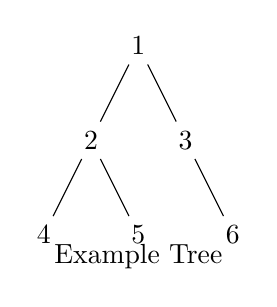
\begin{tikzpicture}[scale=0.8]
        \node {1}
          child {node {2}
            child {node {4}}
            child {node {5}}
          }
          child {node {3}
            child[missing]
            child {node {6}}
          };
        \node[below, draw=none] at (0,-3) {Example Tree};
      \end{tikzpicture}
    \end{column}
  \end{columns}
\end{frame}

\begin{frame}{Binary Trees}
  \begin{definition}
    A \textbf{binary tree} is a tree where each node has at most two children (left and right).
  \end{definition}

  \vspace{0.3cm}

  \begin{columns}
    \begin{column}{0.48\textwidth}
      \textbf{Types of Binary Trees:}
      \begin{itemize}
        \item \textbf{Full}: Every node has 0 or 2 children
        \item \textbf{Complete}: All levels filled except possibly last
        \item \textbf{Perfect}: All internal nodes have 2 children, all leaves at same level
        \item \textbf{Degenerate}: Each node has only one child
      \end{itemize}
    \end{column}
    \begin{column}{0.48\textwidth}
      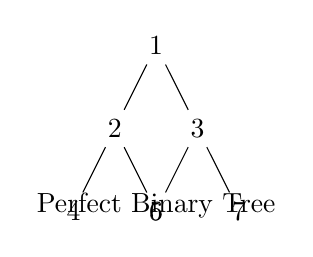
\begin{tikzpicture}[scale=0.7]
        \node {1}
          child {node {2}
            child {node {4}}
            child {node {5}}
          }
          child {node {3}
            child {node {6}}
            child {node {7}}
          };
        \node[below, draw=none] at (0,-2.5) {Perfect Binary Tree};
      \end{tikzpicture}
    \end{column}
  \end{columns}
\end{frame}

\begin{frame}{Binary Search Tree (BST)}
  \begin{definition}
    A \textbf{BST} is a binary tree with ordering property:
    \begin{itemize}
      \item Left subtree contains only nodes with values \textbf{less than} parent
      \item Right subtree contains only nodes with values \textbf{greater than} parent
      \item Both subtrees are also BSTs
    \end{itemize}
  \end{definition}

  \vspace{0.3cm}

  \begin{center}
    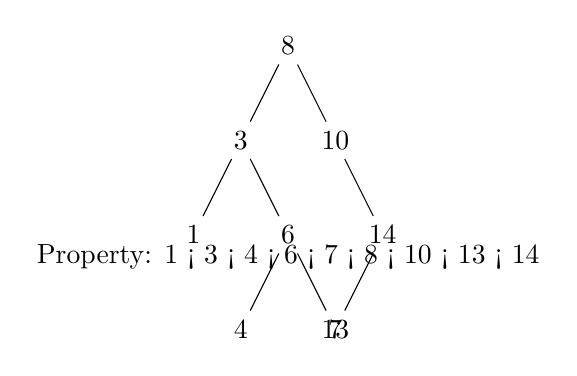
\begin{tikzpicture}[scale=0.8]
      \node {8}
        child {node {3}
          child {node {1}}
          child {node {6}
            child {node {4}}
            child {node {7}}
          }
        }
        child {node {10}
          child[missing]
          child {node {14}
            child {node {13}}
            child[missing]
          }
        };
      \node[below, draw=none] at (0,-3) {Property: 1 < 3 < 4 < 6 < 7 < 8 < 10 < 13 < 14};
    \end{tikzpicture}
  \end{center}
\end{frame}

\begin{frame}[fragile]{BST Operations}
  \begin{columns}
    \begin{column}{0.48\textwidth}
      \begin{block}{Search - O(h)}
        \begin{lstlisting}[language=Python,basicstyle=\tiny\ttfamily]
def search(root, target):
    if root is None or
       root.value == target:
        return root

    if target < root.value:
        return search(root.left,
                     target)
    else:
        return search(root.right,
                     target)
        \end{lstlisting}
      \end{block}
    \end{column}
    \begin{column}{0.48\textwidth}
      \begin{block}{Insert - O(h)}
        \begin{lstlisting}[language=Python,basicstyle=\tiny\ttfamily]
def insert(root, value):
    if root is None:
        return TreeNode(value)

    if value < root.value:
        root.left = insert(
            root.left, value)
    elif value > root.value:
        root.right = insert(
            root.right, value)

    return root
        \end{lstlisting}
      \end{block}
    \end{column}
  \end{columns}

  \vspace{0.3cm}

  \begin{alertblock}{Complexity}
    h = height of tree. Average: O(log n), Worst: O(n) when tree is skewed
  \end{alertblock}
\end{frame}

\begin{frame}{BST vs Array vs Linked List}
  \begin{table}
    \centering
    \begin{tabular}{l|c|c|c}
      \toprule
      \textbf{Operation} & \textbf{Sorted Array} & \textbf{Linked List} & \textbf{BST (balanced)} \\
      \midrule
      Search & O(log n) & O(n) & O(log n) \\
      Insert & O(n) & O(1)* & O(log n) \\
      Delete & O(n) & O(1)* & O(log n) \\
      Min/Max & O(1) & O(n) & O(log n) \\
      Sorted order & Built-in & No & Inorder traversal \\
      \bottomrule
    \end{tabular}
  \end{table}

  \vspace{0.2cm}
  {\small *assuming position is known}

  \vspace{0.3cm}

  \begin{exampleblock}{Applications}
    Databases (indexing), file systems, expression trees, symbol tables, priority queues
  \end{exampleblock}
\end{frame}

% %----------------------------------------------------------------------------------------
% %    TREE TRAVERSALS
% %----------------------------------------------------------------------------------------
\section{Tree Traversals}

\begin{frame}{Depth-First Traversals (DFS)}
  \begin{columns}
    \begin{column}{0.35\textwidth}
      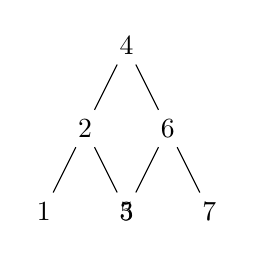
\begin{tikzpicture}[scale=0.7]
        \node {4}
          child {node {2}
            child {node {1}}
            child {node {3}}
          }
          child {node {6}
            child {node {5}}
            child {node {7}}
          };
      \end{tikzpicture}
    \end{column}
    \begin{column}{0.6\textwidth}
      \begin{block}{Three Main Types}
        \begin{enumerate}
          \item \textbf{Inorder} (Left → Root → Right)
            \begin{itemize}
              \item Order: 1, 2, 3, 4, 5, 6, 7
              \item Use: Get sorted values from BST
            \end{itemize}
          \item \textbf{Preorder} (Root → Left → Right)
            \begin{itemize}
              \item Order: 4, 2, 1, 3, 6, 5, 7
              \item Use: Copy tree, serialize
            \end{itemize}
          \item \textbf{Postorder} (Left → Right → Root)
            \begin{itemize}
              \item Order: 1, 3, 2, 5, 7, 6, 4
              \item Use: Delete tree, calculate size
            \end{itemize}
        \end{enumerate}
      \end{block}
    \end{column}
  \end{columns}
\end{frame}

\begin{frame}[fragile]{Inorder Traversal Implementation}
  \begin{columns}
    \begin{column}{0.48\textwidth}
      \begin{block}{Recursive Version}
        \begin{lstlisting}[language=Python,basicstyle=\tiny\ttfamily]
def inorder(root):
    if root is None:
        return []

    result = []
    # Left
    result.extend(
        inorder(root.left))
    # Root
    result.append(root.value)
    # Right
    result.extend(
        inorder(root.right))

    return result
        \end{lstlisting}
      \end{block}
    \end{column}
    \begin{column}{0.48\textwidth}
      \begin{block}{Iterative Version (Stack)}
        \begin{lstlisting}[language=Python,basicstyle=\tiny\ttfamily]
def inorder_iterative(root):
    result = []
    stack = []
    current = root

    while current or stack:
        # Go to leftmost
        while current:
            stack.append(current)
            current = current.left

        # Process node
        current = stack.pop()
        result.append(
            current.value)

        # Visit right
        current = current.right

    return result
        \end{lstlisting}
      \end{block}
    \end{column}
  \end{columns}
\end{frame}

\begin{frame}[fragile]{Breadth-First Traversal (BFS)}
  \begin{columns}
    \begin{column}{0.45\textwidth}
      \begin{block}{Level-Order Traversal}
        Visit nodes level by level, left to right
      \end{block}

      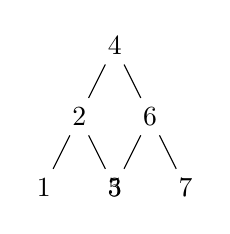
\begin{tikzpicture}[scale=0.6]
        \node {4}
          child {node {2}
            child {node {1}}
            child {node {3}}
          }
          child {node {6}
            child {node {5}}
            child {node {7}}
          };
      \end{tikzpicture}

      Order: 4, 2, 6, 1, 3, 5, 7
    \end{column}
    \begin{column}{0.5\textwidth}
      \begin{lstlisting}[language=Python,basicstyle=\tiny\ttfamily]
from collections import deque

def level_order(root):
    if root is None:
        return []

    result = []
    queue = deque([root])

    while queue:
        node = queue.popleft()
        result.append(node.value)

        if node.left:
            queue.append(node.left)
        if node.right:
            queue.append(node.right)

    return result
      \end{lstlisting}

      \begin{alertblock}{Use Case}
        Shortest path, level processing, check if tree is complete
      \end{alertblock}
    \end{column}
  \end{columns}
\end{frame}

\begin{frame}{Traversal Comparison}
  \begin{table}
    \centering
    \begin{tabular}{l|l|l|l}
      \toprule
      \textbf{Traversal} & \textbf{Order} & \textbf{Use Case} & \textbf{Data Structure} \\
      \midrule
      Inorder & Left-Root-Right & Sorted values (BST) & Stack \\
      Preorder & Root-Left-Right & Copy, serialize & Stack \\
      Postorder & Left-Right-Root & Delete, calculate & Stack \\
      Level-order & Level by level & Shortest path & Queue \\
      \bottomrule
    \end{tabular}
  \end{table}

  \vspace{0.5cm}

  \begin{block}{Complexity}
    \begin{itemize}
      \item \textbf{Time}: O(n) - visit each node once
      \item \textbf{Space}: O(h) for recursion/stack, O(w) for queue (w = max width)
    \end{itemize}
  \end{block}
\end{frame}

% %----------------------------------------------------------------------------------------
% %    HEAPS
% %----------------------------------------------------------------------------------------
\section{Heaps}

\begin{frame}{What is a Heap?}
  \begin{definition}
    A \textbf{heap} is a specialized tree-based data structure that satisfies the \textbf{heap property}, typically implemented as a complete binary tree stored in an array.
  \end{definition}

  \vspace{0.3cm}

  \begin{columns}
    \begin{column}{0.48\textwidth}
      \begin{block}{Min-Heap}
        Parent $\leq$ Children

        \vspace{0.2cm}

        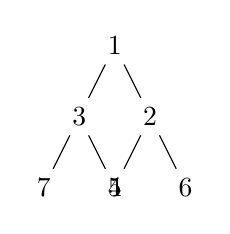
\begin{tikzpicture}[scale=0.6]
          \node {1}
            child {node {3}
              child {node {7}}
              child {node {5}}
            }
            child {node {2}
              child {node {4}}
              child {node {6}}
            };
        \end{tikzpicture}

        Array: [1, 3, 2, 7, 5, 4, 6]
      \end{block}
    \end{column}
    \begin{column}{0.48\textwidth}
      \begin{block}{Max-Heap}
        Parent $\geq$ Children

        \vspace{0.2cm}

        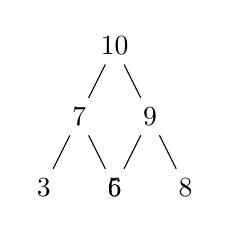
\begin{tikzpicture}[scale=0.6]
          \node {10}
            child {node {7}
              child {node {3}}
              child {node {5}}
            }
            child {node {9}
              child {node {6}}
              child {node {8}}
            };
        \end{tikzpicture}

        Array: [10, 7, 9, 3, 5, 6, 8]
      \end{block}
    \end{column}
  \end{columns}
\end{frame}

\begin{frame}{Heap Array Representation}
  \begin{block}{Index Relationships}
    For a node at index $i$:
    \begin{itemize}
      \item \textbf{Left child}: $2i + 1$
      \item \textbf{Right child}: $2i + 2$
      \item \textbf{Parent}: $\lfloor(i - 1) / 2\rfloor$
    \end{itemize}
  \end{block}

  \vspace{0.3cm}

  \begin{center}
    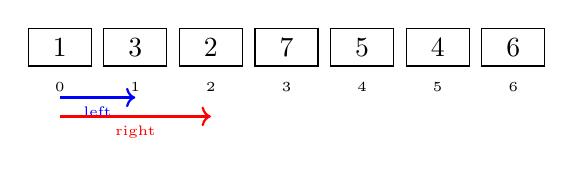
\begin{tikzpicture}[scale=0.8]
      % Array boxes
      \foreach \x/\val in {0/1, 1/3, 2/2, 3/7, 4/5, 5/4, 6/6} {
        \draw (\x*1.2,0) rectangle ++(1,0.6);
        \node at (\x*1.2+0.5,0.3) {\val};
        \node[below] at (\x*1.2+0.5,-0.1) {\tiny\x};
      }

      % Arrows showing parent-child relationships
      \draw[->, thick, blue] (0.5,-0.5) -- (1.7,-0.5);
      \node[below, blue] at (1.1,-0.5) {\tiny left};
      \draw[->, thick, red] (0.5,-0.8) -- (2.9,-0.8);
      \node[below, red] at (1.7,-0.8) {\tiny right};
    \end{tikzpicture}
  \end{center}

  \begin{alertblock}{Efficiency}
    Complete binary tree structure ensures O(log n) height
  \end{alertblock}
\end{frame}

\begin{frame}[fragile]{Heap Operations}
  \begin{columns}
    \begin{column}{0.48\textwidth}
      \begin{block}{Insert - O(log n)}
        \begin{enumerate}
          \item Add to end of array
          \item Bubble up to restore heap property
        \end{enumerate}
        \begin{lstlisting}[language=Python,basicstyle=\tiny\ttfamily]
def insert(self, value):
    self.heap.append(value)
    current = len(self.heap)-1

    while current > 0:
        parent = (current-1)//2
        if self.heap[current] <
           self.heap[parent]:
            self.swap(current,
                     parent)
            current = parent
        else:
            break
        \end{lstlisting}
      \end{block}
    \end{column}
    \begin{column}{0.48\textwidth}
      \begin{block}{Extract Min - O(log n)}
        \begin{enumerate}
          \item Store minimum (root)
          \item Move last element to root
          \item Bubble down to restore heap
        \end{enumerate}
        \begin{lstlisting}[language=Python,basicstyle=\tiny\ttfamily]
def extract_min(self):
    if len(self.heap) == 0:
        raise IndexError()

    min_val = self.heap[0]
    self.heap[0] =
        self.heap.pop()
    self.heapify_down(0)

    return min_val
        \end{lstlisting}
      \end{block}
    \end{column}
  \end{columns}

  \begin{exampleblock}{Peek Min/Max: O(1)}
    Simply return the root element without removing
  \end{exampleblock}
\end{frame}

\begin{frame}{Heap Applications}
  \begin{columns}
    \begin{column}{0.48\textwidth}
      \begin{block}{Priority Queue}
        \begin{itemize}
          \item Task scheduling
          \item CPU scheduling
          \item Event-driven simulation
        \end{itemize}
      \end{block}

      \begin{block}{K Largest/Smallest}
        \begin{itemize}
          \item Use min-heap of size k for k largest
          \item O(n log k) time complexity
        \end{itemize}
      \end{block}
    \end{column}
    \begin{column}{0.48\textwidth}
      \begin{block}{Heapsort}
        \begin{itemize}
          \item Build heap: O(n)
          \item Extract all: O(n log n)
          \item In-place sorting
        \end{itemize}
      \end{block}

      \begin{block}{Graph Algorithms}
        \begin{itemize}
          \item Dijkstra's shortest path
          \item Prim's minimum spanning tree
        \end{itemize}
      \end{block}
    \end{column}
  \end{columns}

  \vspace{0.3cm}

  \begin{alertblock}{Heap vs BST}
    Heap: Quick min/max access, partial order. BST: Full order, any element search
  \end{alertblock}
\end{frame}

% %----------------------------------------------------------------------------------------
% %    BALANCED TREES
% %----------------------------------------------------------------------------------------
\section{Balanced Trees}

\begin{frame}{Why Balanced Trees?}
  \begin{columns}
    \begin{column}{0.48\textwidth}
      \begin{alertblock}{Problem: Unbalanced BST}
        Regular BST can degenerate to linked list

        \vspace{0.2cm}

        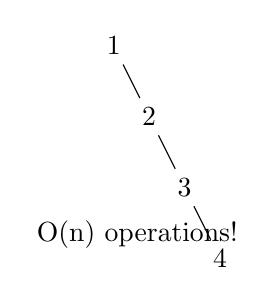
\begin{tikzpicture}[scale=0.6]
          \node {1}
            child[missing]
            child {node {2}
              child[missing]
              child {node {3}
                child[missing]
                child {node {4}}
              }
            };
          \node[below, draw=none] at (0.5,-3.5) {O(n) operations!};
        \end{tikzpicture}
      \end{alertblock}
    \end{column}
    \begin{column}{0.48\textwidth}
      \begin{block}{Solution: Self-Balancing}
        Maintain balanced structure automatically

        \vspace{0.2cm}

        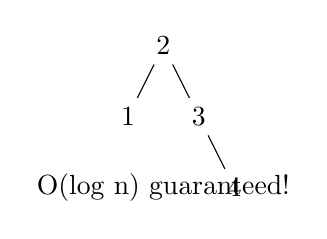
\begin{tikzpicture}[scale=0.6]
          \node {2}
            child {node {1}}
            child {node {3}
              child[missing]
              child {node {4}}
            };
          \node[below, draw=none] at (0,-2.5) {O(log n) guaranteed!};
        \end{tikzpicture}
      \end{block}
    \end{column}
  \end{columns}

  \vspace{0.3cm}

  \begin{exampleblock}{Two Main Approaches}
    \textbf{AVL Trees}: Strictly balanced. \textbf{Red-Black Trees}: Loosely balanced
  \end{exampleblock}
\end{frame}

\begin{frame}{AVL Trees}
  \begin{definition}
    \textbf{AVL tree}: Self-balancing BST where height difference between left and right subtrees is at most 1 for every node.
  \end{definition}

  \begin{block}{Balance Factor}
    BF = height(left subtree) - height(right subtree)

    Must be in \{-1, 0, 1\}. If $|$BF$|$ > 1, rebalancing needed.
  \end{block}

  \vspace{0.3cm}

  \begin{columns}
    \begin{column}{0.48\textwidth}
      \begin{exampleblock}{Rotations}
        \begin{itemize}
          \item Right Rotation (LL case)
          \item Left Rotation (RR case)
          \item Left-Right Rotation (LR case)
          \item Right-Left Rotation (RL case)
        \end{itemize}
      \end{exampleblock}
    \end{column}
    \begin{column}{0.48\textwidth}
      \begin{alertblock}{Properties}
        \begin{itemize}
          \item Height $\leq$ 1.44 log n
          \item Up to 2 rotations per insert
          \item O(log n) rotations for delete
        \end{itemize}
      \end{alertblock}
    \end{column}
  \end{columns}
\end{frame}

\begin{frame}{Red-Black Trees}
  \begin{definition}
    \textbf{Red-Black tree}: Self-balancing BST where each node has a color (red or black) with specific properties.
  \end{definition}

  \begin{block}{Properties}
    \begin{enumerate}
      \item Every node is either red or black
      \item Root is always black
      \item All leaves (NIL) are black
      \item Red nodes cannot have red children
      \item Every path from root to leaf has same number of black nodes
    \end{enumerate}
  \end{block}

  \vspace{0.3cm}

  \begin{alertblock}{Key Differences from AVL}
    \begin{itemize}
      \item Looser balance (height $\leq$ 2 log n)
      \item Faster insert/delete (fewer rotations)
      \item Slightly slower search
    \end{itemize}
  \end{alertblock}
\end{frame}

\begin{frame}{AVL vs Red-Black Comparison}
  \begin{table}
    \centering
    \begin{tabular}{l|c|c}
      \toprule
      \textbf{Feature} & \textbf{AVL Tree} & \textbf{Red-Black Tree} \\
      \midrule
      Balance & Strictly balanced & Loosely balanced \\
      Height & $\leq$ 1.44 log n & $\leq$ 2 log n \\
      Rotations (insert) & Up to 2 & Up to 2 \\
      Rotations (delete) & O(log n) & Up to 3 \\
      Search & Faster & Slightly slower \\
      Insert/Delete & Slower & Faster \\
      Use case & Search-heavy & Insert/delete-heavy \\
      Memory & Less & More (color bit) \\
      \bottomrule
    \end{tabular}
  \end{table}

  \vspace{0.3cm}

  \begin{exampleblock}{Real-world Usage}
    \textbf{AVL}: Database indexing. \textbf{Red-Black}: Java TreeMap, C++ std::map, Linux kernel
  \end{exampleblock}
\end{frame}

% %----------------------------------------------------------------------------------------
% %    GRAPHS
% %----------------------------------------------------------------------------------------
\section{Graphs}

\begin{frame}{Graph Fundamentals}
  \begin{definition}
    A \textbf{graph} G = (V, E) consists of vertices (V) and edges (E) connecting them.
  \end{definition}

  \begin{columns}
    \begin{column}{0.48\textwidth}
      \begin{block}{Graph Types}
        \begin{itemize}
          \item \textbf{Undirected}: Edges have no direction (friendships)
          \item \textbf{Directed}: Edges have direction (follows)
          \item \textbf{Weighted}: Edges have values (distances)
          \item \textbf{Unweighted}: No edge values
        \end{itemize}
      \end{block}
    \end{column}
    \begin{column}{0.48\textwidth}
      \begin{center}
        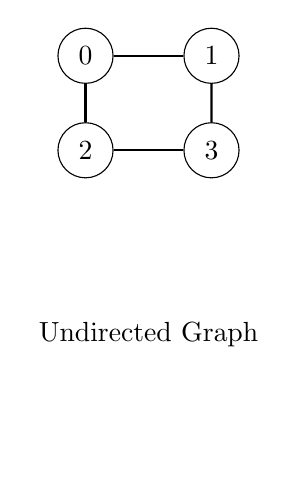
\begin{tikzpicture}[scale=0.8,
          every node/.style={circle, draw, minimum size=7mm}]
          \node (0) at (0,0) {0};
          \node (1) at (2,0) {1};
          \node (2) at (0,-1.5) {2};
          \node (3) at (2,-1.5) {3};

          \draw[thick] (0) -- (1);
          \draw[thick] (0) -- (2);
          \draw[thick] (1) -- (3);
          \draw[thick] (2) -- (3);

          \node[below, draw=none] at (1,-2.5) {Undirected Graph};
        \end{tikzpicture}
      \end{center}
    \end{column}
  \end{columns}
\end{frame}

\begin{frame}{Graph Representations}
  \begin{columns}
    \begin{column}{0.48\textwidth}
      \begin{block}{Adjacency Matrix}
        2D array: matrix[i][j] = 1 if edge exists

        \vspace{0.2cm}

        \begin{tabular}{c|cccc}
          & 0 & 1 & 2 & 3 \\
          \hline
          0 & 0 & 1 & 1 & 0 \\
          1 & 1 & 0 & 0 & 1 \\
          2 & 1 & 0 & 0 & 1 \\
          3 & 0 & 1 & 1 & 0 \\
        \end{tabular}

        \vspace{0.2cm}

        \textbf{Pros}: O(1) edge check

        \textbf{Cons}: O($V^2$) space
      \end{block}
    \end{column}
    \begin{column}{0.48\textwidth}
      \begin{block}{Adjacency List}
        Array of lists: list[i] = neighbors

        \vspace{0.2cm}

        \begin{tabular}{cl}
          0 & $\rightarrow$ [1, 2] \\
          1 & $\rightarrow$ [0, 3] \\
          2 & $\rightarrow$ [0, 3] \\
          3 & $\rightarrow$ [1, 2] \\
        \end{tabular}

        \vspace{0.2cm}

        \textbf{Pros}: O(V + E) space

        \textbf{Cons}: O(V) edge check
      \end{block}
    \end{column}
  \end{columns}

  \vspace{0.3cm}

  \begin{alertblock}{When to Use}
    \textbf{Matrix}: Dense graphs, fast edge lookup. \textbf{List}: Sparse graphs (most real-world)
  \end{alertblock}
\end{frame}

\begin{frame}{Graph Representation Comparison}
  \begin{table}
    \centering
    \begin{tabular}{l|c|c}
      \toprule
      \textbf{Operation} & \textbf{Adjacency Matrix} & \textbf{Adjacency List} \\
      \midrule
      Space & O($V^2$) & O(V + E) \\
      Add edge & O(1) & O(1) \\
      Remove edge & O(1) & O(V) \\
      Check if edge exists & O(1) & O(V) \\
      Find all neighbors & O(V) & O(degree) \\
      Iterate all edges & O($V^2$) & O(V + E) \\
      \bottomrule
    \end{tabular}
  \end{table}

  \vspace{0.3cm}

  \begin{exampleblock}{Space Example}
    Graph with 1000 vertices, 5000 edges:
    \begin{itemize}
      \item Matrix: 1000 $\times$ 1000 = 1,000,000 entries
      \item List: 1000 + 2$\times$5000 = 11,000 entries
      \item List is $\sim$90x more space-efficient!
    \end{itemize}
  \end{exampleblock}
\end{frame}

% %----------------------------------------------------------------------------------------
% %    GRAPH TRAVERSALS
% %----------------------------------------------------------------------------------------
\section{Graph Traversals}

\begin{frame}{Breadth-First Search (BFS)}
  \begin{columns}
    \begin{column}{0.45\textwidth}
      \begin{block}{Algorithm}
        \begin{enumerate}
          \item Start at source vertex
          \item Visit all unvisited neighbors
          \item Then visit neighbors of neighbors
          \item Uses \textbf{Queue} (FIFO)
        \end{enumerate}
      \end{block}
      \begin{center}
        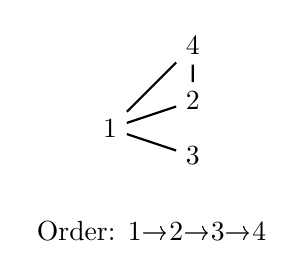
\begin{tikzpicture}[scale=0.7]
          \node (1) at (0,0) {1};
          \node (2) at (1.5,0.5) {2};
          \node (3) at (1.5,-0.5) {3};
          \node (4) at (1.5,1.5) {4};

          \draw[thick] (1) -- (2);
          \draw[thick] (1) -- (3);
          \draw[thick] (1) -- (4);
          \draw[thick] (2) -- (4);

          \node[below, draw=none] at (0.75,-1.5) {Order: 1→2→3→4};
        \end{tikzpicture}
      \end{center}
    \end{column}
%     \begin{column}{0.5\textwidth}
%       \begin{lstlisting}[language=Python,basicstyle=\tiny\ttfamily]
% from collections import deque
% def bfs(graph, start):
%     visited = set()
%     queue = deque([start])
%     visited.add(start)
%     result = []

%     while queue:
%         vertex = queue.popleft()
%         result.append(vertex)

%         for neighbor in
%             graph[vertex]:
%             if neighbor not in
%                visited:
%                 visited.add(neighbor)
%                 queue.append(neighbor)

%     return result
%       \end{lstlisting}
%     \end{column}
  \end{columns}

  \begin{exampleblock}{Applications}
    Shortest path (unweighted), level-order processing, web crawling, social networks
  \end{exampleblock}
\end{frame}

\begin{frame}{Depth-First Search (DFS)}
  \begin{columns}
    \begin{column}{0.45\textwidth}
      \begin{block}{Algorithm}
        \begin{enumerate}
          \item Start at source vertex
          \item Visit unvisited neighbor
          \item Recursively visit that neighbor's neighbors
          \item Backtrack when no unvisited neighbors
          \item Uses \textbf{Stack} (LIFO)
        \end{enumerate}
      \end{block}

      \begin{center}
        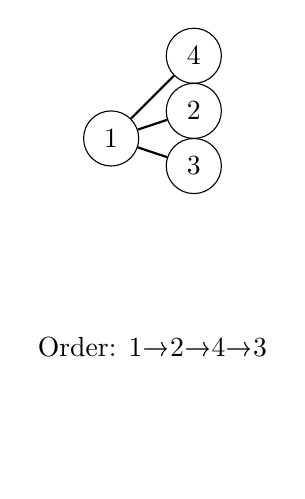
\begin{tikzpicture}[scale=0.7,
          every node/.style={circle, draw, minimum size=7mm}]
          \node (1) at (0,0) {1};
          \node (2) at (1.5,0.5) {2};
          \node (3) at (1.5,-0.5) {3};
          \node (4) at (1.5,1.5) {4};

          \draw[thick] (1) -- (2);
          \draw[thick] (1) -- (3);
          \draw[thick] (1) -- (4);
          \draw[thick] (2) -- (4);

          \node[below, draw=none] at (0.75,-1.5) {Order: 1→2→4→3};
        \end{tikzpicture}
      \end{center}
    \end{column}
%     \begin{column}{0.5\textwidth}
%       \begin{lstlisting}[language=Python,basicstyle=\tiny\ttfamily]
% def dfs_recursive(graph, start,
%                   visited=None):
%     if visited is None:
%         visited = set()

%     visited.add(start)
%     result = [start]

%     for neighbor in graph[start]:
%         if neighbor not in visited:
%             result.extend(
%                 dfs_recursive(
%                     graph, neighbor,
%                     visited))

%     return result
%       \end{lstlisting}

%       \vspace{0.2cm}

%       \begin{alertblock}{Iterative Version}
%         Use explicit stack instead of recursion
%       \end{alertblock}
%     \end{column}
  \end{columns}

  \begin{exampleblock}{Applications}
    Cycle detection, topological sort, connected components, maze solving, backtracking
  \end{exampleblock}
\end{frame}

\begin{frame}{BFS vs DFS}
  \begin{table}
    \centering
    \begin{tabular}{l|c|c}
      \toprule
      \textbf{Feature} & \textbf{BFS} & \textbf{DFS} \\
      \midrule
      Data Structure & Queue & Stack/Recursion \\
      Memory & O(V) - wider & O(h) - deeper \\
      Shortest Path & Yes (unweighted) & No \\
      Completeness & Yes & Yes \\
      Time & O(V + E) & O(V + E) \\
      \bottomrule
    \end{tabular}
  \end{table}

  \vspace{0.3cm}

  \begin{columns}
    \begin{column}{0.48\textwidth}
      \begin{block}{Use BFS for:}
        \begin{itemize}
          \item Shortest path (unweighted)
          \item Level-order processing
          \item Minimum hops/distance
        \end{itemize}
      \end{block}
    \end{column}
    \begin{column}{0.48\textwidth}
      \begin{block}{Use DFS for:}
        \begin{itemize}
          \item Cycle detection
          \item Topological sorting
          \item Finding all paths
        \end{itemize}
      \end{block}
    \end{column}
  \end{columns}
\end{frame}

% %----------------------------------------------------------------------------------------
% %    APPLICATIONS
% %----------------------------------------------------------------------------------------
\section{Applications}

\begin{frame}{Tree Applications}
  \begin{columns}
    \begin{column}{0.48\textwidth}
      \begin{block}{File Systems}
        \begin{itemize}
          \item Directories and files form tree
          \item Root directory at top
          \item Recursive size calculation
        \end{itemize}
      \end{block}

      \begin{block}{HTML DOM}
        \begin{itemize}
          \item Each HTML tag is a node
          \item Parent-child relationships
          \item Tree traversal for rendering
        \end{itemize}
      \end{block}
    \end{column}
    \begin{column}{0.48\textwidth}
      \begin{block}{Database Indexes}
        \begin{itemize}
          \item B-Trees and B+ Trees
          \item Fast range queries
          \item O(log n) search/insert/delete
        \end{itemize}
      \end{block}

      \begin{block}{Decision Trees (ML)}
        \begin{itemize}
          \item Classification and regression
          \item Each node is a decision
          \item Leaves are outcomes
        \end{itemize}
      \end{block}
    \end{column}
  \end{columns}

  \vspace{0.3cm}

  \begin{exampleblock}{More Applications}
    Abstract syntax trees (compilers), Huffman coding (compression), expression evaluation
  \end{exampleblock}
\end{frame}

\begin{frame}{Graph Applications}
  \begin{columns}
    \begin{column}{0.48\textwidth}
      \begin{block}{Social Networks}
        \begin{itemize}
          \item Vertices: Users
          \item Edges: Friendships/Follows
          \item BFS: Degrees of separation
          \item DFS: Connection exploration
        \end{itemize}
      \end{block}

      \begin{block}{Maps \& Navigation}
        \begin{itemize}
          \item Vertices: Locations
          \item Edges: Roads (weighted)
          \item Dijkstra's: Shortest path
          \item Applications: GPS, routing
        \end{itemize}
      \end{block}
    \end{column}
    \begin{column}{0.48\textwidth}
      \begin{block}{Web Page Ranking}
        \begin{itemize}
          \item Vertices: Web pages
          \item Edges: Hyperlinks
          \item PageRank algorithm
          \item Google's foundation
        \end{itemize}
      \end{block}

      \begin{block}{Course Prerequisites}
        \begin{itemize}
          \item Vertices: Courses
          \item Edges: Prerequisites
          \item Topological sort: Valid order
          \item Cycle detection: Invalid prereqs
        \end{itemize}
      \end{block}
    \end{column}
  \end{columns}

  \vspace{0.3cm}

  \begin{exampleblock}{More Applications}
    Network flow, dependency resolution, recommendation systems, circuit design
  \end{exampleblock}
\end{frame}

\begin{frame}{When to Use Trees vs Graphs}
  \begin{columns}
    \begin{column}{0.48\textwidth}
      \begin{block}{Use Trees When:}
        \begin{itemize}
          \item Hierarchical relationships
          \item One path between any two nodes
          \item Clear parent-child structure
          \item No cycles allowed
        \end{itemize}

        \vspace{0.2cm}

        \textbf{Examples:}
        \begin{itemize}
          \item File systems
          \item DOM
          \item Organizational charts
          \item Expression trees
        \end{itemize}
      \end{block}
    \end{column}
    \begin{column}{0.48\textwidth}
      \begin{block}{Use Graphs When:}
        \begin{itemize}
          \item Many-to-many relationships
          \item Multiple paths between nodes
          \item Network-like structure
          \item Cycles may exist
        \end{itemize}

        \vspace{0.2cm}

        \textbf{Examples:}
        \begin{itemize}
          \item Social networks
          \item Maps and roads
          \item Web links
          \item Dependencies
        \end{itemize}
      \end{block}
    \end{column}
  \end{columns}
\end{frame}

% %----------------------------------------------------------------------------------------
% %    SUMMARY
% %----------------------------------------------------------------------------------------
\section{Summary}

\begin{frame}{Key Takeaways}
  \begin{block}{Trees}
    \begin{itemize}
      \item Binary trees, BSTs: O(log n) operations when balanced
      \item Traversals: Inorder (sorted), Preorder (copy), Postorder (delete), Level-order (BFS)
      \item Heaps: Priority queue, O(1) peek, O(log n) insert/extract
      \item Balanced trees (AVL, Red-Black): Guaranteed O(log n)
    \end{itemize}
  \end{block}

  \begin{block}{Graphs}
    \begin{itemize}
      \item Adjacency matrix (dense) vs list (sparse)
      \item BFS: Shortest path, level-order, queue-based
      \item DFS: Cycle detection, topological sort, stack-based
      \item Both: O(V + E) time complexity
    \end{itemize}
  \end{block}

  \begin{block}{Applications Everywhere}
    File systems, databases, social networks, maps, compilers, machine learning, web ranking
  \end{block}
\end{frame}

\begin{frame}{Complexity Summary}
  \begin{table}
    \centering
    \small
    \begin{tabular}{l|c|c|c}
      \toprule
      \textbf{Data Structure} & \textbf{Search} & \textbf{Insert} & \textbf{Delete} \\
      \midrule
      BST (balanced) & O(log n) & O(log n) & O(log n) \\
      BST (worst) & O(n) & O(n) & O(n) \\
      AVL Tree & O(log n) & O(log n) & O(log n) \\
      Red-Black Tree & O(log n) & O(log n) & O(log n) \\
      Heap (min/max) & O(n) & O(log n) & O(log n) \\
      Heap (peek) & O(1) & - & - \\
      \bottomrule
    \end{tabular}
  \end{table}

  \vspace{0.3cm}

  \begin{alertblock}{Graph Traversals}
    BFS and DFS both have O(V + E) time complexity
  \end{alertblock}
\end{frame}

\begin{frame}[plain]
  \begin{center}
    {\Huge Thank You!}

    \vspace{1cm}

    {\large Questions?}
  \end{center}
\end{frame}

\end{document}
